\documentclass{article}

\usepackage{polski} % Pozwala na użycie polskiego. Ustawia między innymi fontenc na T1
\usepackage[utf8]{inputenc} % Informuje o kodowaniu

\usepackage{graphicx}
\graphicspath{ {./Obrazy/} }

\usepackage{textcomp} % Znaki specjalne takie jak ~

\title{Laboratorium sieci komputerowych - c2 \\ Konfiguracja interfejsów sieciowych}
\author{Krzysztof Dąbrowski gr. 3}
\date{\today}

\begin{document}
\maketitle{}
\tableofcontents{}
%\newpage

\section{Cel zajęć}
Celem pierwszej części zajęć c2 było odwzorowanie schematu sieci na stacji roboczej. By to osiągnąć trzeba było wykreować maszyny wirtualne oraz odpowiednie interfejsy sieciowe.

\begin{figure}[h]
    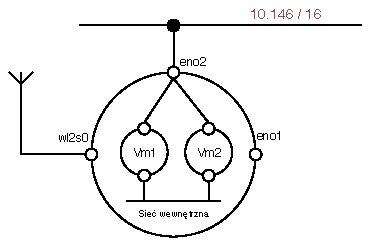
\includegraphics[width=0.80\textwidth]{schemat}
    \centering
    \caption{Schemat sieci do wykreowania}
    \label{fig:schemat}
\end{figure}

\section{Zbadanie lokalnych interfejsów}
Dzięki poleceniu \texttt{ifconfig} można uzyskać informacje o interfejsach gospodarza. Uzyskanie w tens sposób nazwy interfejsów zostały naniesione na schemat \ref{fig:schemat}.



\end{document}